% !TeX spellcheck = da_DK
\subsection{Referencespænding til offset}\label{subsec:Spaendingsref}
\subsubsection{Teori og design}
Der skal forsynes med en konstant spænding til offsetjusteringen, da denne skal anvendes som sammenligningsgrundlag ift. inputsignalet. Denne konstante spænding kaldes en referencespænding og består af en spændingsforsyning, en modstand og en spændingsreferencediode. Der anvendes en referencediode (LM385), som både findes som $1.2$V og $2.5$V. Et eksempel på en opsætning af en spændingsreference kan ses på \figref{fig:Spaendingsreference}.

\begin{figure}[H]
	\centering
	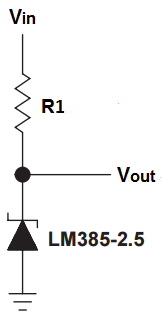
\includegraphics[scale=0.7]{figures/cProblemloesning/ReferenceEksempel.PNG}
	\caption{På figuren ses et eksempel på en opsætning af et kredsløb for en spændingsreference med LM$385$. \textit{(Revideret)} \cite{Instruments2005}}
	\label{fig:Spaendingsreference}
\end{figure}

\noindent For at udregne værdien af modstanden R1 på \figref{fig:Spaendingsreference} anvendes følgende generelle formel:
\begin{equation}
R1 = \dfrac{V_{forsyning} - V_{Reference}}{I_{Z}}
\end{equation}
\noindent Hvor $V_{forsyning}$ er forsyningsspændingen, som sendes ind i kredsløbet, $V_{Reference}$ er den referencespænding, der skal sendes ud af systemet, og $I_{Z}$ er strømforbruget fra de komponenter, som er i referencespændingskredsløbet. \\
Først udregnes R$1$ for referencespændingen. $V_{forsyning}$ er de $5.5$V, der forsynes med fra spændingsforsyningen, og $V_{Reference}$ er $2.5$V. I kredsløbet for offsettet indgår en operationsforstærker (TL$081$), der har en maksimal biasstrøm på $10$nA \cite{Corporation1995}. Referencedioden har et arbejdsområde mellem $20\mu$A til $20m$A og for at sikre, at der er strøm nok til referencedioden, er den sat til at bruge $200\mu$A \cite{Instruments2005}. Dermed kan strømforbruget $I_{Z}$ udregnes som summen af de to biasstrømme. Alle de kendte værdier indsættes i formlen:
\begin{equation}
R1 = \frac{5.5V - 2.5V}{0.0002 + (1 \cdot 10^{-8A})} = 14999.2500\Omega \approx 15K\Omega
\end{equation}  
Da offsettet i accelerometeret er på $1.6325$V, jævnført afsnit \ref{Sec_Pilot_Data} på side \pageref{Sec_Pilot_Data}, skal referenceværdi ligeledes være $1.6325$V. For at opnå denne referenceværdi bruges indsættes en spændingsdeler efter referencedioden, som vil levere $2.5$V. Den generelle formel for en spændingsdeler er: 
\begin{equation} \label{eq:Spaendingsdeler}
V_{out} = V_{in} \cdot \dfrac{R3}{R2 + R3}
\end{equation}

R$2$ i \eqref{eq:Spaendingsdeler} bliver valgt til at være $10$K$\Omega$. Derudover er $V_{out}$ $1.6325$V, $V_{in}$ er $2.5$V. Ligningen kommer altså til at være således: 
\begin{equation}
1.6325V = 2.5 \cdot \dfrac{R3}{10000\Omega + R3} \\
R3 = 18818.4438\Omega \approx 18820\Omega
\end{equation}

\subsubsection{Simulering}
Der foretages en simulering i LTspice af spændingsreferencen og spændingsdeleren for at undersøge, om de opfylder de opstillede krav. På \figref{fig:Spaendingsreference_offset} ses simuleringen af spændingsreferencen med spændingsdeler. 

\begin{figure}[H]
	\centering
	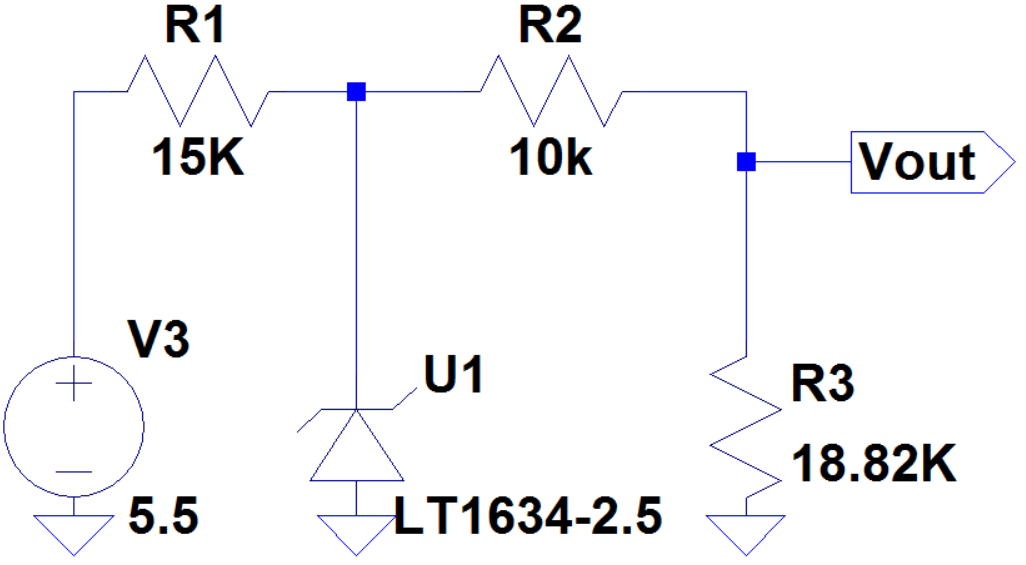
\includegraphics[scale=.5]{figures/cProblemloesning/OffsetSpaendingsRef2.PNG}
	\caption{Opsætning af kredsløbet for en spændingsreference til offsettet. Hvor der først er en spændingsreference efterfølgt at en spændingsdeler, som gør at outputtet fra spændingsreferencen på $2.5$V bliver til $1.6325$V. }
	\label{fig:Spaendingsreference_offset}
\end{figure}

\noindent Resultatet af simuleringen kan ses i \tableref{Tab:SpaendigsRef_offset}:
\begin{table}[H]
\centering
\begin{tabular}{|l|l|l|l|}\hline
    & \textit{\begin{tabular}[c]{@{}l@{}}Forventet\\outputsignal\end{tabular}} & \textit{\begin{tabular}[c]{@{}l@{}}Målte\\outputsignal\end{tabular}} & \textit{Afvigelse} \\ \hline
\textit{\begin{tabular}[c]{@{}l@{}}Input fra\\spændingsforsyning\end{tabular}}      & $5.5$V             &   $5.5$V      &   $0\%$         \\ \hline
\textit{\begin{tabular}[c]{@{}l@{}}Output fra\\spændingsreference\end{tabular}}     & $2.5$V             &  $2.5007$V    &   $0.03 \%$    \\ \hline
\textit{\begin{tabular}[c]{@{}l@{}}Output fra\\spændingsdeler\end{tabular}}         & $1.6325$V          &  $1.6330$V    &   $0.03 \%$     \\ \hline
\end{tabular}
\caption{I tabellen ses resultaterne fra simuleringen i LTspice af spændingsreferencen med spændingsdeleren.}
\label{Tab:SpaendigsRef_offset}
\end{table}
\noindent I \tableref{Tab:SpaendigsRef_offset} fremgår det, at der er en lav afvigelse mellem det forventede output og det simulerede output. Dette forventes, da der benyttes ideelle komponenter i LTspice. Derved fungerer kredsløbet teoretisk og kan implementeres.

\subsubsection{Implementering og test}\label{spaendingsref_resultat}
I implementeringen arbejdes der med reelle komponenter. Derfor antages det, at der kan være afvigelser fra resultaterne imellem testen med ideelle komponenter i dette afsnit og testen med reelle komponenter i simuleringen. \\
Der ses på \figref{fig:Spaendingsreference_offset}, at der skal benyttes tre modstande på hhv. $15$K$\Omega$, $10$K$\Omega$ og $18820 \Omega$ til opbygningen af spændingsreferencen og spændingsdeleren til offsettet. Der findes ikke en $18.820$K$\Omega$, hvorfor en $18$K$\Omega$ modstand i serie med en $820\Omega$ modstand benyttes. Disse blev målt inden testen, hvilket fremgår i \tableref{Tab:modstand_offset}.

\begin{table}[H]
	\centering
	\begin{tabular}{|l|l|l|}
		\hline
		\textit{Teoretisk} & \textit{Ved måling} & \textit{\% afvigelse} \\ \hline
		$15$K$\Omega$       & $15002\Omega$      & $0.013$\%               \\ \hline
		$10$K$\Omega$       & $10003.6\Omega$    & $0.036$\%               \\ \hline
		$18$K$\Omega$       & $17966.3\Omega$    & $0.187$\%               \\ \hline
		$820\Omega$         & $818.08\Omega$     & $0.234$\%               \\ \hline
	\end{tabular}
	\caption{I tabellen ses der, at alle fire modstande afviger lidt fra deres teoretiske værdi, hvilket er forventet af reelle komponenter. Kravet til disse fire modstande var dog, at de maks må afvige fra deres teoretiske værdi med $\pm1\%$ jævnfør afsnit \ref{Ref_Offset_Afs} på side \pageref{Ref_Offset_Afs}. Disse modstande accepteres derfor.}
	\label{Tab:modstand_offset}
\end{table}
\noindent Herefter implementeres kredsløbet. Til aflæsning af spændingsniveauerne anvendes et multimeter. De aflæste resultater står i \tableref{Tab:SpaendingsRef_offset_test}.
\begin{table}[H]
\centering
\begin{tabular}{|l|l|l|l|} \hline
                              & \textit{\begin{tabular}[c]{@{}l@{}}Forventet\\outputsignal\end{tabular}} & \textit{\begin{tabular}[c]{@{}l@{}}Målte\\outputsignal\end{tabular}} & \textit{Afvigelse} \\ \hline
\textit{\begin{tabular}[c]{@{}l@{}}Input fra\\spændingsforsyning\end{tabular}}       & $5.5$V    & $5.550$V  & $0.91 \%$ \\ \hline
\textit{\begin{tabular}[c]{@{}l@{}}Output fra\\spændingsreference\end{tabular}}      & $2.5$V    & $2.499$V  & $0.04 \%$ \\ \hline
\textit{\begin{tabular}[c]{@{}l@{}}Output fra\\spændingsdeler\end{tabular}}          & $1.6325$V & $1.6296$V & $0.18 \%$ \\ \hline
\end{tabular}
\caption{I tabellen ses en oversigt over de forventede og målte outputsignaler fra testen for spændingsreferencen og spændingsdeleren til offsetjustering.}
\label{Tab:SpaendingsRef_offset_test}
\end{table}
%Ud fra \tableref{Tab:SpaendingsRef_offset_test} ses det, at afvigelserne for inputtet fra spændingsreferencen har en lidt større afvigelse end de andre. Dette kan skyldes, at spændingsforsyningen ikke er ideel og derfor kan variere lidt i dens outputspænding. Variationen fra spændingsforsyningen vil ikke have en indflydelse, hvis den ikke varierer mere end det målte. Outputtet fra spændingsreferencen accepteres, da afvigelsen er på $0.04 \%$. Det samme gælder for outputtet af spændingsdeleren, hvor afvigelsen er på $0.18 \%$. 
Der ses ud fra resultaterne i \tableref{Tab:SpaendingsRef_offset_test}, at spændingsreferencen samt spændingsdeleren overholder kravene fra afsnit \ref{Ref_Offset_Afs} på side \pageref{Ref_Offset_Afs}. Derudover ligger afvigelserne indenfor tolerancerne. \\
Outputimpedansen overholder dog ikke kravet, da den er:
\begin{equation}
R_{eq} = \dfrac{(R2 \cdot R3)}{R2 + R3} \Longrightarrow \dfrac{10000 \cdot 18820}{10000 + 18820} = 6530.19\Omega \approx 6.53K\Omega
\end{equation}
Da inputimpedansen i den inverterende kanal i operationsforstærkeren i offsetjusteringen har en indgangsimpedans på $100$K$\Omega$, vil forholdet imellem output- og inputimpedans i koblingen være problematisk. Der vil dannes en spændingsdeling imellem R$3$ og den pågældende modstand, som sidder inden den inverterende kanal. Dermed vil signalet variere alt efter inputsignalet til operationsforstærkeren i offsetjusteringens ikke-inverterende kanal. Løsningen på problematikken i denne kobling er, at indsætte en buffer. Signalet fra spændingsdeleren sendes ind i bufferens ikke-inverterende kanal, hvorfor outputimpedansen ikke er relevant, da denne kanal har en indgangsimpedans på $10^{12}\Omega$. Outputimpedansen fra bufferen vil være meget lav, og derfor vil koblingen imellem denne blok og offsetjusteringen være mulig. Der benyttes en operationsforstærker TL081 i en ikke konverterende konfiguration og med et gain på $1$. Dette ses på \figref{fig:Buffer}. \fxnote{Kilde på buffer}
\begin{figure}[H]
	\centering
	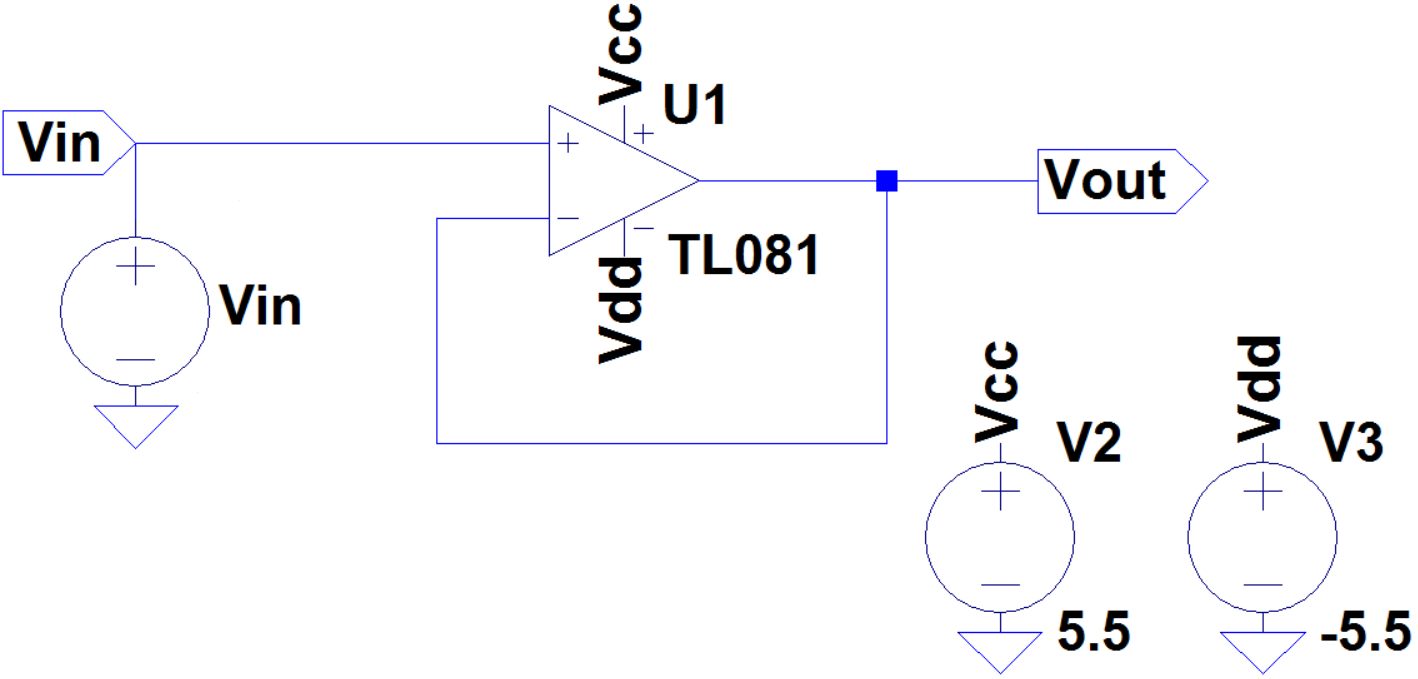
\includegraphics[scale=0.4]{figures/cProblemloesning/Buffer_LT.png}
	\caption{På figuren ses en buffer, som fungerer som en forstærker med et gain på faktor 1.}
	\label{fig:Buffer}
\end{figure}
Herved kan blokken accepteres og benyttes til videre implementering.